% Chapter Template

\chapter{M\'etodos} % Main chapter title

\label{Chapter3} % Change X to a consecutive number; for referencing this chapter elsewhere, use \ref{ChapterX}

%----------------------------------------------------------------------------------------
%	SECTION 1
%----------------------------------------------------------------------------------------

\section{Descripci\'on general}

Como se mencion\'o anteriormente, este trabajo se enfoca en extraer informaci\'on sobre los vasos sangu\'ineos oculares en pos de la detecci\'on de enfermedades que pueden reflejarse en los mismos utilizando angiograf\'ias fluorescentes.
Las im\'agenes con fluoresc\'ina carecen de ruido debido a colores y cuestiones \'opticas por su naturaleza, pero a su vez poseen ruido generado por la cantidad de vasos que se encuentra por debajo de la retina en la coroide.\\
Con motivo de realizar un mejor an\'alisis sobre las im\'agenes buscamos, en primer instancia, reducir el ruido de las mismas enfocandonos en realzar los vasos de la retina por sobre los de la coroide. Con esto en mente buscamos algoritmos de preprocesamiento que nos acerquen a lo que buscamos para analizar su comportamiento y poder determinar cual ser\'ia el mas adecuado para preprocesar las im\'agenes antes de extraer la informaci\'on necesaria.

\section{Preprocesamiento}
\subsection{¿Por qu\'e?}
Al analizar los diferentes m\'etodos de captura de la retina podemos observar que en cada una de ellos, aunque en diferentes formas, existe ruido generado por la misma tecnolog\'ia de captura. Para poder lograr un resultado \'optimo debemos ser capaces de llevar el ruido mencionado al nivel m\'inimo posible. Para lograrlo se utilizan distintos algoritmos de preprocesamiento, cada uno de ellos mas o menos eficiente dependiendo del tipo de ruido que exista en la im\'agen.\\
\\
Como objetivos principales del preprocesamiento podemos destacar:
\begin{description}
  \item[Reducci\'on de ruido:] Eliminaci\'on de diferencias de intensidad que son generados por ruido producido generalmente por los elementos de captura de la im\'agen.
  \item[Realce de bordes:] Realzar los bordes para luego facilitar la detecci\'on de los mismos en la etapa de segmentaci\'on.
  \item[Suavizado de im\'agenes:] Permite normalizar las intensidades de los p\'ixeles que estan fuera de la \"normalidad\" del vecindario donde se encuentra.
\end{description}

\subsection{Algoritmos investigados}

Luego de realizar un an\'alisis de investigaci\'on acerca de los algoritmos de preprocesamiento existentes encontramos que aquellos que mejor se adaptaban a las necesidades de nuestra casu\'istica eran aquellos que respetaban los bordes al suavizar la im\'agen.\\
\\
Por un lado analizamos los algoritmos mas adecuados para la eliminaci\'on del fondo de la im\'agen, para este fin decidimos analizar tanto la mediana como la media. Por el otro, buscamos algoritmos para la reducci\'on de ruido para im\'agenes de angiodraf\'ia fluorescente y decidimos quedarnos con el algoritomo de difusi\'on anisotr\'opica y el filtro de coherencia.

\subsubsection{Remoci\'on fondo}

Para la remoci\'on de fondo se utilizaron dos filtros diferentes, por un lado el filtro de media y por el otro un filtro de mediana. Tanto la media como la mediana son filtros de paso bajo, es decir, un filtro que aten\'ua las intensidades altas y mantienen las intensidades bajas. Este tipo de filtros intentan reducir el ruido suavizando. En nuestro caso, al ser utilizado con grandes ventanas, nos permiten obtener una imagen homogénea que podemos restar a la imagen original para remover el fondo.

\begin{description}
  \item[Media:] La media, como su nombre lo indica, realiza un promedio entre las instensidades vecinas al p\'ixel llevando a cabo una convoluci\'on y utiliza el resultado para actualizar el valor del mismo.
  \item[Mediana:] Por otro lado, la mediana es un filtro no lineal dado que depende de un algoritmo de ordenamiento para determinar cu\'al es el valor que divide a la mitad al conjunto, al encontrarlo utiliza este para actualizar el valor del p\'ixel analizado.
\end{description}

\subsubsection{Reducci\'on de ruido}

Para la reducci\'on de ruido nos enfocamos en encontrar filtros que nos permitieran suavizar y eliminar ruido pero siempre intentando no perder los borde y objetos de inter\'es de la imagen. Para esto buscamos filtros que puedan orientarse en las direcciones de los bordes y de esta manera mantenerlos con contrastes altos\\
\\En nuestra b\'usqueda encontramos varios algoritmos matem\'aticos que apuntaban en esta direcci\'on como el filtro gaussiano pero determinamos que no estaban plenamente enfocados en mantener las estructuras sino mas bien que esto era una consecuencia de su naturaleza. Sobre el final de la misma, y a trav\'es de la lectura de algunas investigaciones descubrimos el filtro de difusi\'on anisotr\'opica \cite{perona1990scale} y el filtro de coherencia \cite{weickert1999coherence}.

\begin{description}
  \item[Difusi\'on anisotr\'opica:]
  \item[Filtro de coherencia:]
\end{description}

\subsection{Resultados obtenidos}

En pos de exponer de manera adecuada los resultados obtenidos de los experimentos realizados proponemos graficar los mismos pero no sin antes explicar como se obtuvieron.\\
\\En todos los casos la metodolog\'ia que se utiliz\'o fu\'e realizar pruebas exhaustivas variando dos par\'ametros: cantidad de iteraciones de los filtros y el tamaño de ventana de la remoci\'o de fondo.\\
\\En ambos casos se relev\'o un rango que se considero suficiente dado que luego de el límite establecido se noto que a grandes pasos los resultados solo deca\'ian en calidad.\\

\begin{figure}[H]
	\centering
	\begin{subfigure}[b]{0.48\textwidth}
        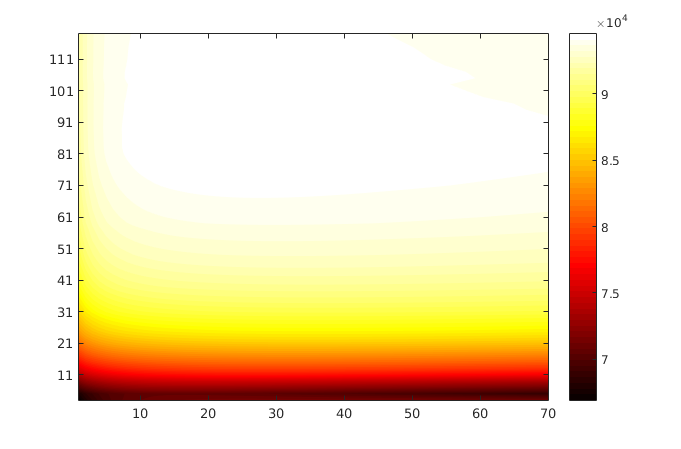
\includegraphics[width=1\textwidth]{./Figures/AllDataThermalAnisodiff.png}
        \caption{Mapa completo}
        \label{fig:thermalforanisodiffwithmediana}
  \end{subfigure}
  \begin{subfigure}[b]{0.48\textwidth}
        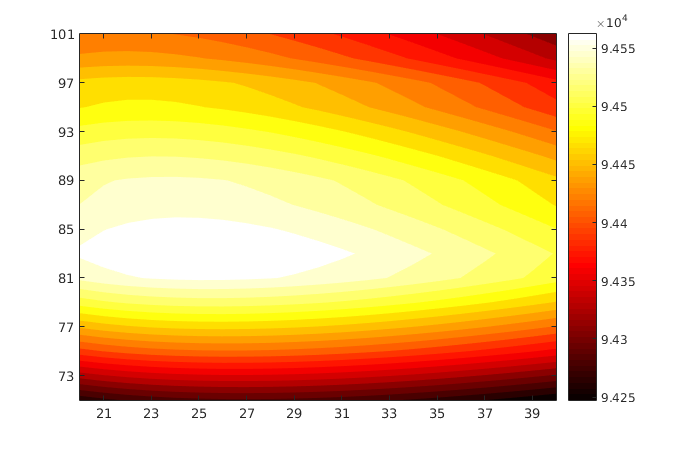
\includegraphics[width=1\textwidth]{./Figures/CenteredThermalAnisodiff.png}
        \caption{Centrado en la zona mas intensa}
        \label{fig:thermalforanisodiffwithmedianacentered}
  \end{subfigure}
	\label{fig:thermalfigure}
	\caption{Mapa de calor utilizando Mediana y Filtro Anisotr\'opico}
\end{figure}

Dada la naturaleza de los experimentos decidimos que la mejor manera de mostrar los resultados era un mapa de calor(Figura \ref{fig:thermalforanisodiffwithmediana}) y para poder visualizar mejor el comportameniento en la zona de calor mas intenso aislamos la regi\'on (Figura \ref{fig:thermalforanisodiffwithmedianacentered}) y lo graficamos en tres dimensiones (Figura \ref{fig:centeredregionthermal}).\\

\begin{figure}[H]
	\centering
  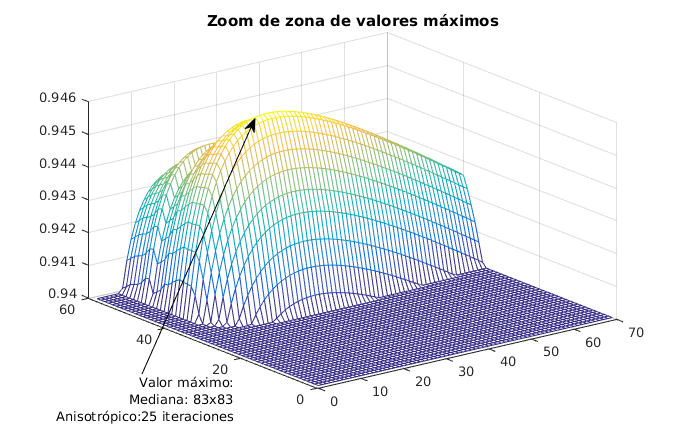
\includegraphics[width=0.75\textwidth]{./Figures/FiguraEvaluacionMaximosAnisodiff.png}
  \caption{Regi\'on \'optima graficada en tres dimensiones}
  \label{fig:centeredregionthermal}
\end{figure}


FALTAN EXPERIMENTOS:
\begin{description}
  \item[Media con anisodiff] En algun momento descartamos la media pero no tenemos datos guardados para mostrar
  \item[Media con coherencia] En algun momento descartamos la media pero no tenemos datos guardados para mostrar
  \item[Mediana con coherencia] Hicimos el de difusion anistropica, y el de coherencia pudimos buscarle la vuelta ahora para hacerlo mas rapido
\end{description}

\subsection{Comparativa}

Pendiente de los resultados de los experimentos.

\section{Extracci\'on de caracter\'isticas}

\section{M\'etodo de segmentaci\'on}
